\documentclass[12pt,letterpaper]{article}
\usepackage[utf8]{inputenc}
\usepackage[spanish]{babel}
\usepackage{amsmath}
\usepackage{amsfonts}
\usepackage{float}
\usepackage{amssymb}
\usepackage{graphicx}
\usepackage[left=2cm,right=2cm,top=2cm,bottom=2cm]{geometry}
\usepackage{pdfpages}
\usepackage{subfigure}
\author{}
\date{}

\begin{document}
%insertar portada

\includepdf{figuras/Caratula}

%\tableofcontents

%En este trabajo se explicará cómo realizar una presentación de un proyecto para los trabajos de laboratorio de la materia \textbf{Interfaces}.

\section{Introducción}
Utilizando la técnica de LGR (Lugar Geométrico de las Raíces), analizar el comportamiento de estabilidad del siguiente sistema, que representa el modelo matemático de un motor de CC al cual se le aplica un control del tipo P-D (Proporcional + Derivativo, en el cual la accion derivativa se realiza sobre la señal de salida del sistema).
\begin{figure}[H]
\centering
\subfigure[Esquema de sistema completo.]
{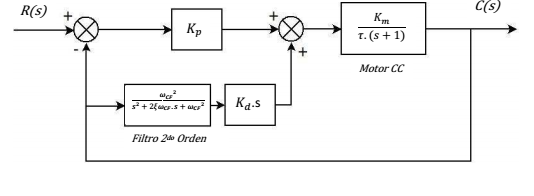
\includegraphics[width=12 cm]{figuras/fig1.png}}
\end{figure}
Teniendo en cuenta los siguientes valores:
\begin{enumerate}
\item[•]$K_{m}=1,53$
\item[•]$\tau=0.00254$
\item[•]$\omega_{cf}=100 . \pi$
\item[•]$\xi=0.9$
\end{enumerate}
\section{Simplificación del Sistema}
El análisis comienza calculando la Función de Transferencia equivalente del lazo derivativo, si se denomina los subsistemas $L_{1}= K_{d}.s$ y $L_{2}=\frac{\omega_{cf}^{2}}{s^{2}+2 \xi \omega_{cf}+\omega_{cf}^{2}}$, y se nombra la expresión correspondiente al motor de CC como $M = \frac{K_{m}}{\tau s+1}$. Luego, $L=L_{1}.L{2}$, a continuación, la Función de Transferencia equilavente en el lazo derivativo es: $F_{e} = \frac{M}{1-M.L} $.
La siguiente figura ilustra el diagrama de bloques resultante:
\begin{figure}[H]
\centering
\subfigure[Esquema de sistema simplificado.]
{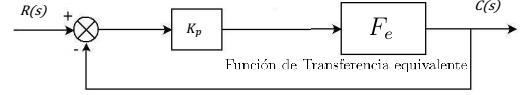
\includegraphics[width=12 cm]{figuras/fig2.png}}
\end{figure}
\section{Obtención del Lugar Geométrico de las Raíces}
Sobre el archivo de Matlab adjunto se desarrolla el código que permite obtener el Lugar Geómetrico de las Raices del Sistema, es importante tener en cuenta que su forma varía de acuerdo al valor de la constante derivativa del controlador, por lo tanto se analiza el comportamiento de cada caso particular.
\subsection{Lugar Geométrico de las Raíces para Kd=-11.65}
Al asignar un valor inferior a $K_{d}=-11.65$ se observa que el LGR correspondiente comienza sobre valores ubicados sobre el semiplano derecho de s, lo cual implica que para valores pequeños de ganancia $K_{p}$, los polos dominantes en lazo cerrado del Sistema se ubican sobre dicho semiplano, provocando la inestabilidad del sistema.
Sin embargo cabe destacar que para valores crecientes de $K_{p}$ es posible configurar un Sistema estable, debido a que las ramas que corresponden a los polos dominantes del sistema recorren una trayectoria que cruza al eje imaginario y circulan hacia el semiplano izquierdo. 
%La siguiente FIGURITA ilustra el LGR para $K_{d}=-12$.
%\begin{figure}[H]
%\centering
%\subfigure[LGR para $K_{d}=-12$.]
%{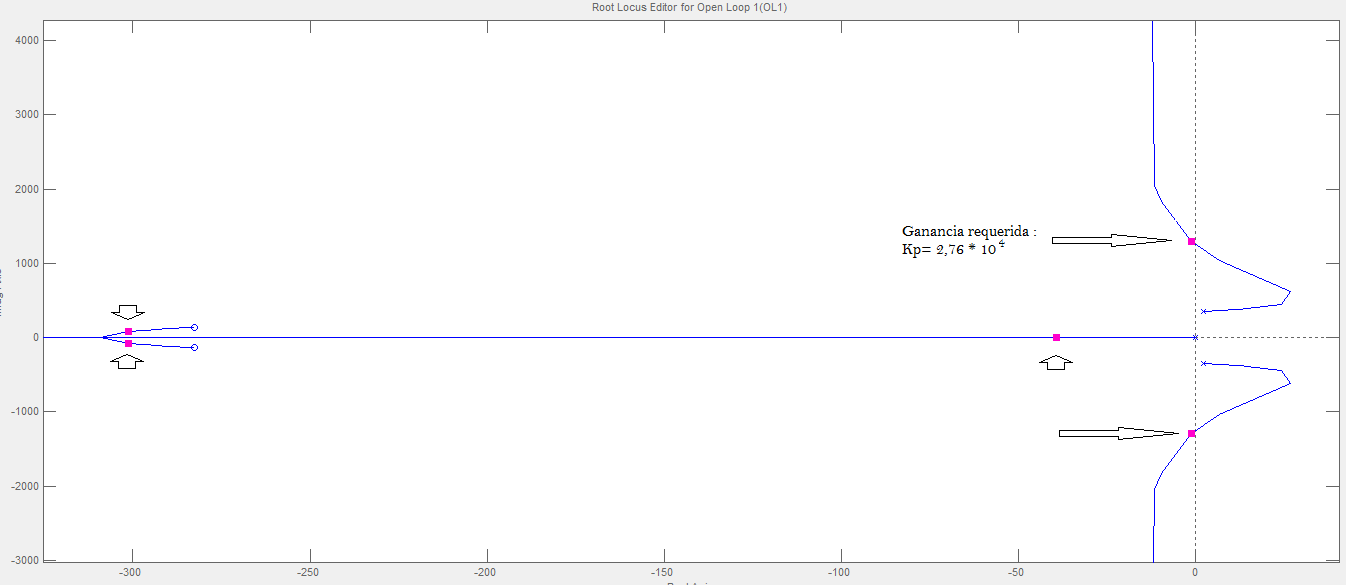
\includegraphics[width=16 cm]{figuras/fig3.png}}
%\end{figure}
%Es posible aproximar el análisis de dicho sistema, a un sistema equivalente de Segundo Orden, debido a que el polo superior ubicado inmediatamente a continuación de los polos dominantes (aproximadamente ubicado en -40 + 0j), se encuentra lo suficientemente lejos, de manera que es posible afirmar que su influencia en la Respuesta del Sistema es despreciable.

Cuando $K_{d}$ adquiere esta magnitud, el Sistema se encuentra en una situación crítica,ya que los polos dominantes de lazo abierto del Sistema se encuentran ubicados aproximadamente sobre el eje imaginario, además, la trayectoria que recorren sus respectivas ramas, inicialmente circulan hacia el semiplano derecho. Es posible afirmar ante esta situación, que para valores pequeños $K_{d}$ el Sistema se torna inestable.
En particular si $K_{p}$ adquiere magnitudes pequeñas, resulta interesante analizar el comportamiento del Sistema a través del Criterio de Nyquist, utilizando Matlab para calcular la posición de los polos de lazo abierto, y la posición de los polos en lazo cerrado (para una ganancia $K_{p}$ definida), la siguiente figura ilustra, el LGR del Sistema para $K_{d}=-11.65$ y la posición de los polos de lazo cerrado para $K_{p}=0.5$, además se muestra el correspondiente Diagrama de Nyquist y la Respuesta al Escalon del Sistema.

\begin{figure}[H]
\centering
\subfigure[LGR para $K_{d}=-11.65$. Diagrama de polos y ceros, Diagrama de Nyquist, Respuesta al Escalón; para $K_{p}=0.5$.]
{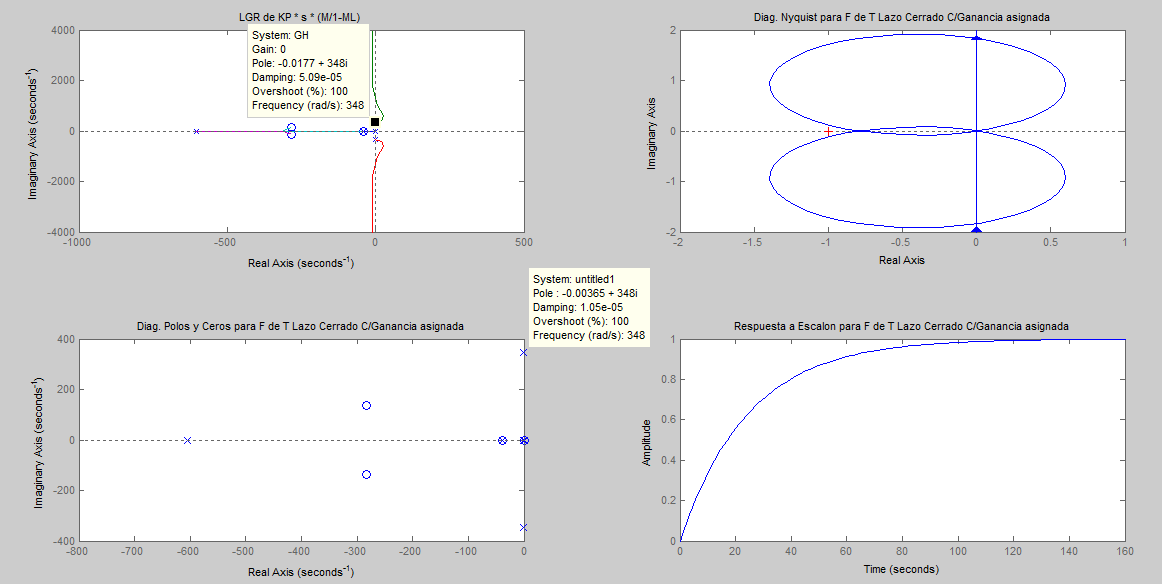
\includegraphics[width=18 cm]{figuras/fig_ns1.png}}
\end{figure}

Se puede observar los siguientes hechos característicos:
\begin{enumerate}
\item[•] Los polos del sistema en lazo abierto se encuentran ubicados sobre el semiplano izquierdo, sin embargo al estar tan cerca del eje imaginario, las ramas cruzan dicho eje para valores muy pequeños de $K_{p}$.
\item[•] Para una ganancia $K_{p}=0.5$, los polos dominantes en lazo cerrado se encuentran sobre el semiplano izquierdo, lo cual implica que al utilizar el Criterio de Nyquist P=0. Sobre dicho diagrama, no se establecen revoluciones alrededor de -1, por lo tanto N=0. En consecuencia no hay polos del Sistema en Lazo Cerrado ubicados sobre el semiplano derecho, lo cual implica que el sistema es estable.

\end{enumerate} 

En el caso que $K_{p}=1$, se provoca la inestabilidad del Sistema, debido a que se producen 2 revoluciones alrededor de -1 en sentido horario entonces N=-2; como no hay polos de lazo abierto ubicados sobre el semiplano derecho, P=0, luego existen Z=2 polos de lazo cerrado ubicados en el semiplano derecho; como consecuencia; el sistema es inestable. Cabe destacar la importancia que adquiere el Criterio de Nyquist, ya que al realizar la gráfica de la Respuesta al Escalon, la forma de la curva resultante no ilustra de forma clara un comportamiento inestable. La siguiente figura ilustra el LGR , junto con el Diagrama de Nyquist y el Diagrama de polos y ceros del Sistema en Lazo Cerrado, esta última grafica nos muestra que los polos dominantes del Sistema en Lazo Cerrado se encuentran sobre el semiplano derecho.

\begin{figure}[H]
\centering
\subfigure[LGR para $K_{d}=-11.65$. Diagrama de polos y ceros, Diagrama de Nyquist, Respuesta al Escalón; para $K_{p}=1$.
Se destaca la posición de los polos de segundo orden de lazo cerrado del Sistema.]
{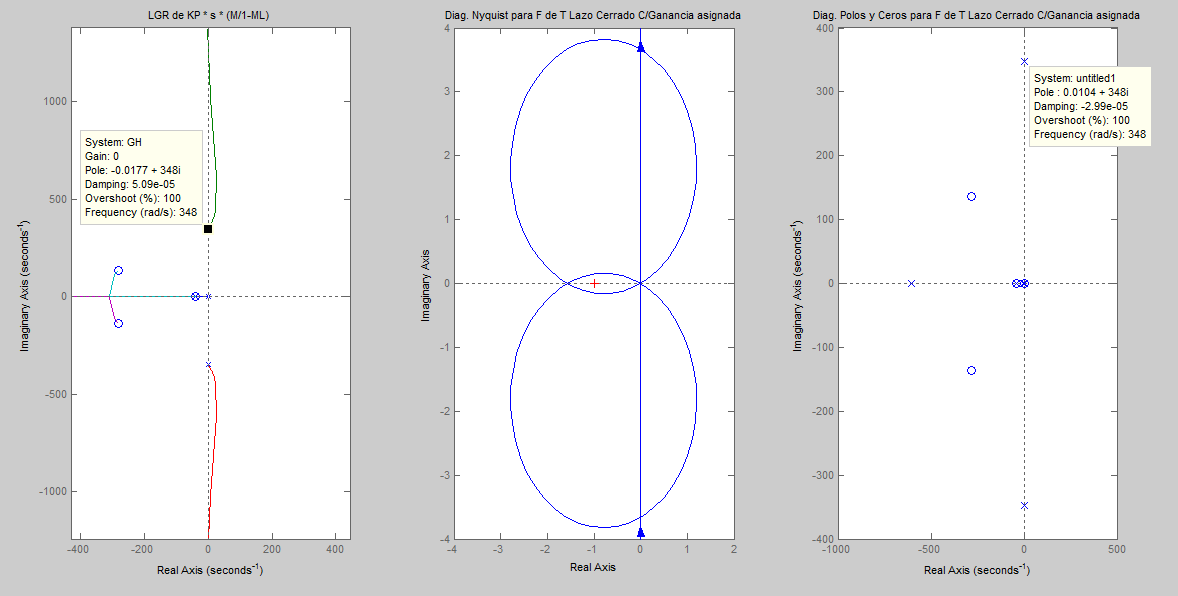
\includegraphics[width=15 cm]{figuras/fig_ns2.png}}
\end{figure}

Para valores de ganancia considerablemente grandes, se establece la estabilidad del Sistema, debido a la dirección que recorren las ramas de los polos dominantes del Sistema.

\subsection{Lugar Geométrico de las Raíces para Kd=-2}
Al asignar un valor a $K_{d}=-2$ se observa que el LGR correspondiente describe un comportamiento de un Sistema de Segundo Orden cuya Respuesta corresponde a un Sistema Sobreamortiguado, debido a que para valores de ganancia $K_{p}$ crecientes, los polos dominantes del sistema se encuentran sobre el eje real, a continuación se ilustra el LGR del Sistema, y la Respuesta al Escalón del Sistema.

\begin{figure}[H]
\centering
\subfigure[LGR para $K_{d}=-2$. Respuesta al Escalón; para valores crecientes de $K_{p}$.]
{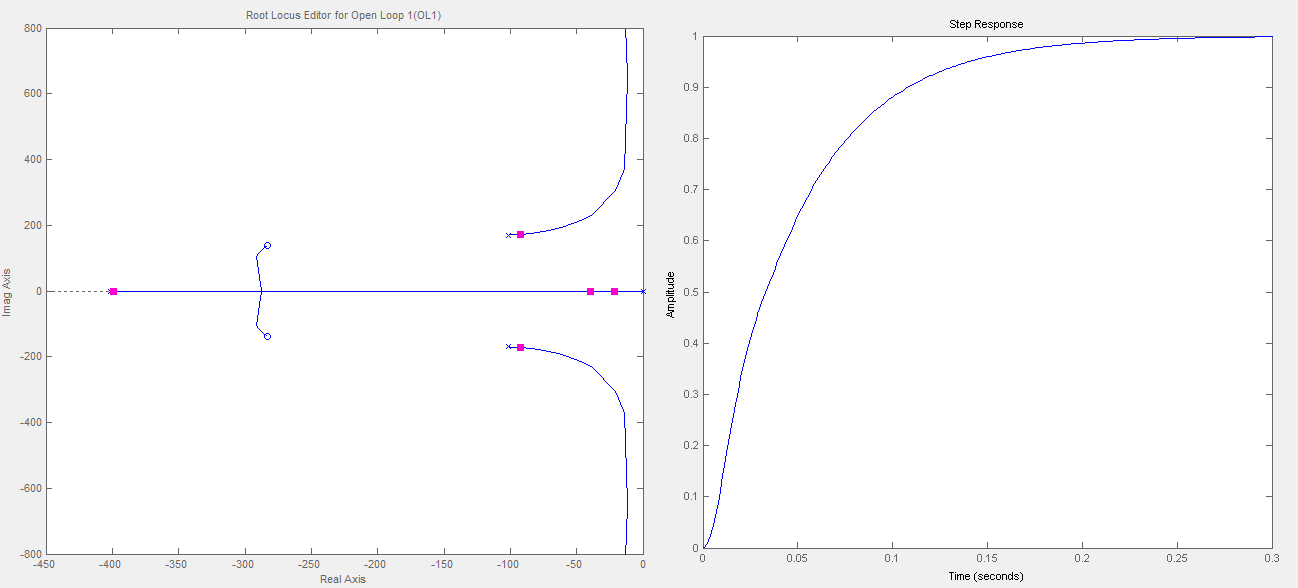
\includegraphics[width=15 cm]{figuras/fig_ns3.png}}
\end{figure}

A medida que la ganancia $K_{p}$ crece, un polo de orden superior se aproxima a la parte real del par de polos complejos conjugados del Sistema, de manera que afecta a la posibilidad para justificar la aproximación a un Sistema de Segundo Orden.

A continuación se ilustra la Respuesta al Escalón del Sistema, cuando el polo de orden superior se aproxima hacia el par de polos complejos conjugados.

\begin{figure}[H]
\centering
\subfigure[Efecto de la Respuesta al Escalón; debido a cercanía de polo de orden superior sobre los polos complejos cojugados.]
{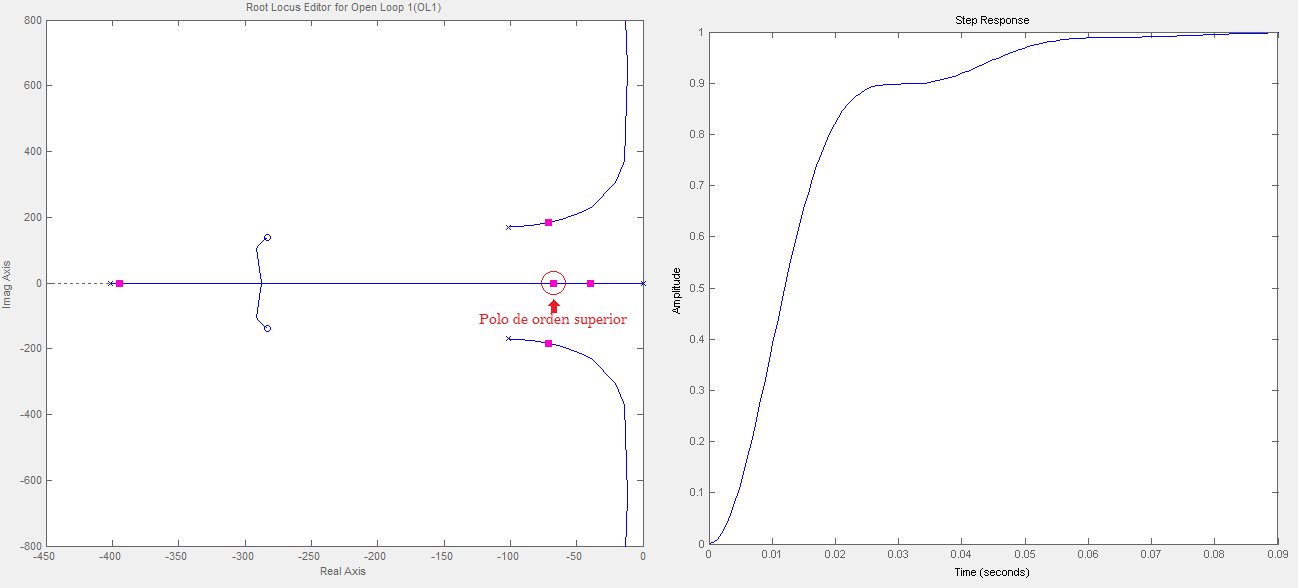
\includegraphics[width=15 cm]{figuras/fig_ns4.png}}
\end{figure}

Para ganancias superiores, es posible realizar la aproximación hacia el análisis de un Sistema de Segundo Orden, gracias a la lejanía de el polo de orden superior mas cercano al par de polos dominantes, es importante destacar que este Sistema se mantiene estable para todos los valores de ganancia $K_{p}$, debido a que las ramas que corresponden a los polos complejos conjugados, no cruzan el eje imaginario.

En este caso, la curva de la Respuesta corresponde a la Respuesta Subamortiguada, a medida que la ganancia tiende a valores muy grandes, se mantiene constante el tiempo de asentamiento, mientras que la magnitud del tiempo pico disminuye.

\subsection{Lugar Geométrico de las Raíces para Kd=0.65}
Al asignar un valor superior a $K_{d}=0.65$ se observa que el LGR correspondiente comienza sobre valores ubicados sobre el semiplano derecho de s, lo cual implica que para valores pequeños de ganancia $K_{p}$, los polos dominantes en lazo cerrado del Sistema se ubican sobre dicho semiplano, provocando la inestabilidad del sistema.
Sin embargo cabe destacar que para valores crecientes de $K_{p}$ es posible configurar un Sistema estable, debido a que las ramas que corresponden a los polos dominantes del sistema recorren una trayectoria que cruza al eje imaginario y circulan hacia el semiplano izquierdo. 

Al asignar un valor a $K_{d}=0.65$ se observa que el LGR correspondiente describe un comportamiento de un Sistema de Segundo Orden cuya Respuesta corresponde a un Sistema Sobreamortiguado, debido a que para valores de ganancia $K_{p}$ infinitesimalmente pequeños, los polos dominantes del sistema se encuentran sobre el eje real, a continuación se ilustra el LGR del Sistema.

\begin{figure}[H]
\centering
\subfigure[LGR para $K_{d}=0.65$.]
{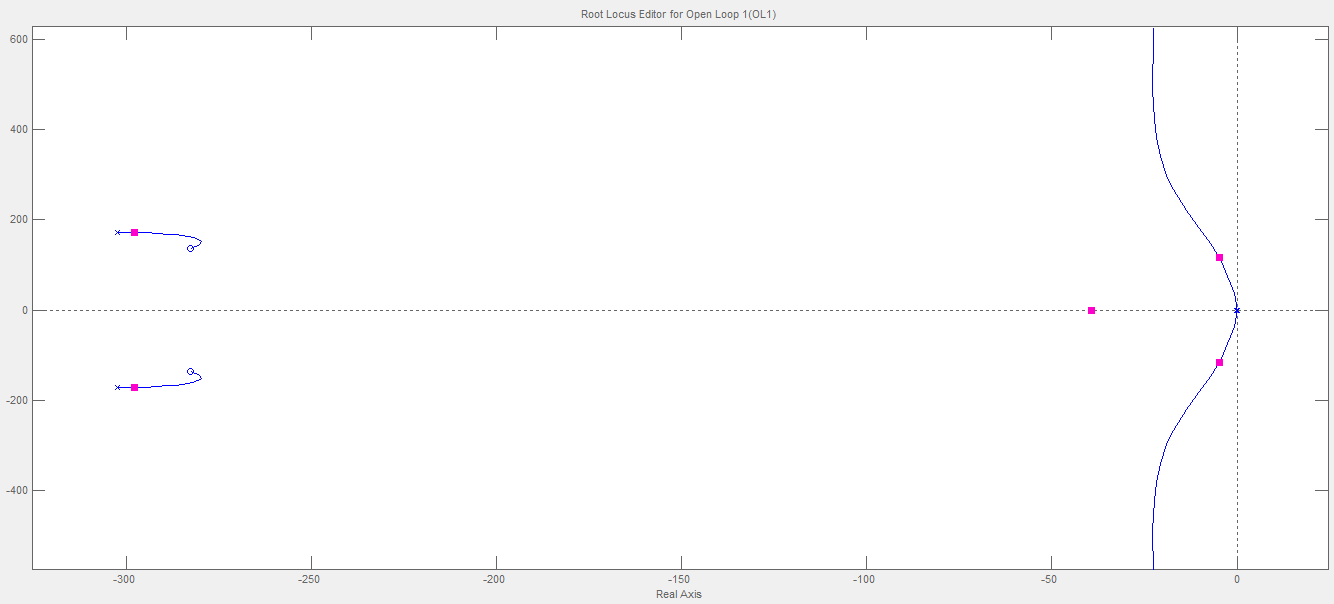
\includegraphics[width=15 cm]{figuras/fig_ns5.png}}
\end{figure}

A partir de la observación del Lugar Geométrico de las Raices del sistema resultante es posible afirmar que siempre permanece en estado estable cuando la ganancia $K_{p}$ varía. Además, la lejanía del polo de orden superior que se ubica sobre la izquierda de los polos dominantes, se encuentra lo suficientemente lejos de la parte real de los mismos, permitiendo la justificación de la aproximación a un Sistema de Segundo Orden, cuya forma de la Respuesta al Escalón corresponde a un Sistema Subamortiguado.

\section{Conclusiones}
El problema propuesto resultó enriquecedor debido a que ilustra la influencia de los parámetros de los controladores PID, en este caso en particular $K_{p}$ y $K_{d}$, brinda un ejemplo de la importancia que adquiere un previo análisis antes de la configuración de los parámetros de un sistema, y además integra muchos conceptos que se aprendieron en la materia, tales como: Operaciones Algebraicas con los Diagramas de Bloque, Análisis de la Respuesta de Sistemas de Segundo Orden, Análisis de Estabilidad mediante el Criterio de Nyquist, Análisis mediante el Lugar Geométrico de las Raíces (para la descripción cualitativa del comportamiento del Sistema a medida que $K_{p}$ varía, y la influencia del valor de $K_{d}$ sobre las ubicaciones de los polos en lazo abierto del Sistema). 

\end{document}

